\documentclass{book}
\usepackage{physics}
\usepackage{graphicx}
\usepackage{caption}
\usepackage{amsmath}
\usepackage{bm}
\usepackage{authblk}
\usepackage{empheq}
\usepackage[shortlabels]{enumitem}
\usepackage{amsfonts}
\usepackage{esint}
\usepackage[makeroom]{cancel}
\usepackage{dsfont}
\usepackage{centernot}
\usepackage{mathtools}
\usepackage{bigints}
\usepackage{amsthm}
\theoremstyle{definition}
\newtheorem{defn}{Definition}[section]
\newtheorem{prop}{Proposition}[section]
\newtheorem{rmk}{Remark}[section]
\newtheorem{thm}{Theorem}[section]
\newtheorem{exmp}{Example}[section]
\newtheorem{prob}{Problem}[section]
\newtheorem{sln}{Solution}[section]
\newtheorem*{prob*}{Problem}
\newtheorem{exer}{Exercise}[section]
\newtheorem*{exer*}{Exercise}
\newtheorem*{sln*}{Solution}
\usepackage{empheq}
\usepackage{hyperref}
\usepackage{tensor}
\usepackage{xcolor}
\hypersetup{
	colorlinks,
	linkcolor={black!50!black},
	citecolor={blue!50!black},
	urlcolor={blue!80!black}
}


\usepackage{qcircuit}




\newcommand*\widefbox[1]{\fbox{\hspace{2em}#1\hspace{2em}}}

\newcommand{\p}{\partial}
\newcommand{\R}{\mathbb{R}}
\newcommand{\C}{\mathbb{C}}
\newcommand{\lag}{\mathcal{L}}
\newcommand{\nn}{\nonumber}
\newcommand{\ham}{\mathcal{H}}
\newcommand{\M}{\mathcal{M}}
\newcommand{\I}{\mathcal{I}}
\newcommand{\K}{\mathcal{K}}
\newcommand{\F}{\mathcal{F}}
\newcommand{\w}{\omega}
\newcommand{\lam}{\lambda}
\newcommand{\al}{\alpha}
\newcommand{\be}{\beta}
\newcommand{\x}{\xi}


\newcommand{\sig}{\bm\sigma}
\newcommand{\n}{\mathbf{n}}
\newcommand{\X}{\mathbf{X}}
\newcommand{\s}{\mathbf{S}}

\newcommand{\G}{\mathcal{G}}

\newcommand{\f}[2]{\frac{#1}{#2}}

\newcommand{\ift}{\infty}

\newcommand{\lp}{\left(}
\newcommand{\rp}{\right)}

\newcommand{\lb}{\left[}
\newcommand{\rb}{\right]}

\newcommand{\lc}{\left\{}
\newcommand{\rc}{\right\}}


\newcommand{\V}{\mathbf{V}}
\newcommand{\U}{\mathbf{U}}
\newcommand{\Id}{\mathbb{I}}
\newcommand{\D}{\mathcal{D}}
\newcommand{\Z}{\mathbf{Z}}
\newcommand{\had}{\mathbf{H}}
\newcommand{\Y}{\mathbf{Y}}
%\setcounter{chapter}{-1}


\makeatletter
\renewcommand{\@chapapp}{Part}
%\renewcommand\thechapter{$\bf{\ket{\arabic{chapter}}}$}
%\renewcommand\thesection{$\bf{\ket{\arabic{section}}}$}
%\renewcommand\thesubsection{$\bf{\ket{\arabic{subsection}}}$}
%\renewcommand\thesubsubsection{$\bf{\ket{\arabic{subsubsection}}}$}
\makeatother



\usepackage{subfig}
\usepackage{listings}
\captionsetup[lstlisting]{margin=0cm,format=hang,font=small,format=plain,labelfont={bf,up},textfont={it}}
\renewcommand*{\lstlistingname}{Code \textcolor{violet}{\textsl{Mathematica}}}
\definecolor{gris245}{RGB}{245,245,245}
\definecolor{olive}{RGB}{50,140,50}
\definecolor{brun}{RGB}{175,100,80}
\lstset{
	tabsize=4,
	frame=single,
	language=mathematica,
	basicstyle=\scriptsize\ttfamily,
	keywordstyle=\color{black},
	backgroundcolor=\color{gris245},
	commentstyle=\color{gray},
	showstringspaces=false,
	emph={
		r1,
		r2,
		epsilon,epsilon_,
		Newton,Newton_
	},emphstyle={\color{olive}},
	emph={[2]
		L,
		CouleurCourbe,
		PotentielEffectif,
		IdCourbe,
		Courbe
	},emphstyle={[2]\color{blue}},
	emph={[3]r,r_,n,n_},emphstyle={[3]\color{magenta}}
}


\begin{document}
\begin{titlepage}\centering
 \clearpage
 \title{{\textsc{\textbf{QUANTUM INFORMATION \& QUANTUM COMPUTATION}}}\\ \smallskip - A Quick Guide - \\}
 \author{\bigskip Huan Q. Bui}
  \affil{Colby College\\$\,$\\ PHYSICS \& MATHEMATICS\\ Statistics \\$\,$\\Class of 2021\\}
 \date{\today}
 \maketitle
 \thispagestyle{empty}
\end{titlepage}

\subsection*{Preface}
\addcontentsline{toc}{subsection}{Preface}

Greetings,\\

This guide is based on \textit{Quantum Computer Science, An Introduction} by N. David Mermin, and \textit{Quantum Computation and Quantum Information} by Isaac Chuang and Michael Nielsen. \\

The entire copy of this text can be found in Chapter 4 of \textit{Quantum Theories, A Quick Guide to}. While this text fits under the more general title of \textit{quantum theories}, the topics covered here are no longer physical phenomena as explained by quantum theories. Rather, we will pay much attention to what happens when computation and information theory meet quantumness. This guide thus deserves its status as a separate set of notes.\\

This text has two parts. Part 1 covers many topics in an introductory manner. These include the ``rules of the game'' and some simple applications and problems. Most of Part 1 will be based on \textit{Quantum Computer Science: An Introduction} by Mermin, even though I might pull some topics from Mike and Ike. Part 2 contains more problems and topics in greater and more advanced details. Most of this part will be based on \textit{Quantum Computation and Quantum Information} by Mike and Ike. Part 1 should serve as an introduction to part 2. \\

I will assume familiarity with linear algebra. There will be a section on some potentially unfamiliar linear algebra, but I would like to keep it short.\\

Enjoy!

\newpage
\tableofcontents
\newpage



\chapter{An Introduction}

\newpage


\section{Linear Algebra}

\subsection{Bases \& Linear Independence}
\subsection{Linear Operators \& Matrices}
\subsection{The Pauli Matrices}
\subsection{Inner Products}
\subsection{Eigenvectors \& Eigenvalues}
\subsection{Adjoints \& Hermitian Operators}
\subsection{Tensor Products}
\subsection{Operator Functions}
\subsection{Commutators \& Anti-commutators}
\subsection{Polar \& Singular Value Decomposition}
\newpage
\section{Quantum Mechanics}
\subsection{The Postulates}
\subsection{State space}
\subsection{Evolution}
\subsection{Quantum Measurement}
\subsection{Distinguishing quantum states}
\subsection{Projective Measurements}
\subsection{POVM measurements}
\subsection{Phase}
\subsection{Composite Systems}
\subsection{A global view}
\subsection{Superdense coding}
\newpage
\section{The Density Operator}
\subsection{Ensembles of Quantum States}
\subsection{General Properties of the Density Operator}
\subsection{The Reduced Density Operator}
\subsection{The Schmidt Decomposition \& Purifications}
\subsection{EPR \& the Bell Inequality}

\newpage

\section{Introduction}

\subsection{Quantum computer}

Quantum mechanics dictates most (if not all) physical interactions. Classical computers work \textit{because} of quantum mechanics. What makes quantum computers ``quantum'' is the fact that the program \textit{completely} controls \textit{all} interactions in the physical system that makes up the computer. External, unaccounted for, interactions are destructive, resulting in what we call \textit{decoherence}. \\

Decoherence occurs when the system could not be completely isolated from its own irrelevant interactions. Thus, it is out of the necessity to eliminate decoherence that individual bits must be microscopic systems such as quantum states of atoms. 




\subsection{Cbits}

\subsubsection{Cbits, Cbit states, Brakets \& Vectors}

A \textit{bit} in a classical computer contains either a 0 or a 1. A classical computer stores this information in a physical system, such as a switch, which can be either ON or OFF. Such a two-state physical system is called a \textit{Cbit}. The quantum generalization of a Cbit is called a \textit{Qbit} (or \textit{qubit}). \\

The Cbit can either be in the \textit{state} $\ket{0}$ or $\ket{1}$. The state of five Cbits 11001, say, is given by $\ket{1}\ket{1}\ket{0}\ket{0}\ket{1}$, where putting the kets together like this implies the use of the \textit{tensor product}. We won't worry too much about that for now. \\

Two Cbits can be in any of the following $2^2$ states:
\begin{align}
\ket{1}\ket{1}, \quad \ket{1}\ket{0}, \quad \ket{0}\ket{1}, \quad \ket{0}\ket{0}.
\end{align}
Similarly, three Cbits can be in any of their respective $2^3$ states
\begin{align}
\ket{1}\ket{1}\ket{1}, \ket{1}\ket{1}\ket{0},\dots,\ket{0}\ket{0}\ket{0}.
\end{align}

To simplify notations, we will just write $\ket{A}\ket{B} = \ket{AB}$ from now on. We can also shorten our notations to represent integers in various bases, but we won't pay much attention to that here. \\

So far we have been looking at \textit{basis states} of the Cbits. These basis states are orthonormal vectors in some finite dimensional vector space. For example, in the single Cbit case, the vector space is two-dimensional (since there are exactly two basis states), spanned by 
\begin{align}
\ket{0} \equiv \begin{pmatrix}
1 \\0
\end{pmatrix},\quad 
\ket{1} \equiv \begin{pmatrix}
0 \\ 1
\end{pmatrix}.
\end{align}
A larger number of Cbits requires an exponentially larger vector space to describe. For example, the basis states for Cbits are 
\begin{align}
\ket{11} &\equiv \ket{1} \otimes \ket{1}\nn\\
\ket{10} &\equiv \ket{1} \otimes \ket{0}\nn\\
\ket{01} &\equiv \ket{0} \otimes \ket{1}\nn\\
\ket{00} &\equiv \ket{0} \otimes \ket{0}\nn.
\end{align}
The funny $\otimes$ symbol denotes the tensor product. Actually \textit{evaluating} tensor products is merely book-keeping. For example:
\begin{align}
\begin{pmatrix}
a\\b
\end{pmatrix}\otimes
\begin{pmatrix}
c\\d
\end{pmatrix}
=
\begin{pmatrix}
a\begin{pmatrix}
c\\d
\end{pmatrix}
\\
b\begin{pmatrix}
c\\d
\end{pmatrix}
\end{pmatrix}
=
\begin{pmatrix}
ac\\ad\\bc\\bd
\end{pmatrix}.
\end{align} 
This generalizes to tensor products of matrices as well, as we will see. Note that in mathematics the tensor product is done in a slightly different order, but there is no fatal discrepancy to worry about. The truly remarkable aspect of the tensor product is that it works. It is not obvious at all how, say
\begin{align}
\ket{5}_3 = \ket{101} = 
\begin{pmatrix}
0\\1
\end{pmatrix}\otimes
\begin{pmatrix}
1\\0
\end{pmatrix}\otimes
\begin{pmatrix}
0\\1
\end{pmatrix}
=
\begin{pmatrix}
0\\0\\0\\0\\0\\1\\0\\0
\end{pmatrix},
\end{align}
where the subscript 3 in $\ket{\,\,}_3$ denotes the number of Cbits, has the property that the number 5 in the 3-Cbit system is represented by a vector whose only nonzero entry is in the 5$^{\text{th}}$ position. If it's not clear what's going on, I would suggest verifying that 
\begin{align}
\ket{j}_n \equiv \begin{pmatrix}
0\dots 1 \dots 0
\end{pmatrix}^\top 
\end{align}
where the number 1 is at the $j^\text{th}$ position, and the resulting vector lives in a $2^n$-dimensional vector space over the finite field $\mathbb{F}_2 = \{0,1\}$. \\

In general, the tensor product allows us to represent the state $\ket{m}_n$ as a $2^n$ column vector whose entries are zero except at the $m^{\text{th}}$ entry where the entry is 1. \\

We can also turn this rule around and obtain a compact, product state representation of any number $x$ where $0 \leq x < 2^n$. We won't go into the details here. 









\subsection{Reversible operations on Cbits}

Most quantum operations are \textit{reversible}, exceptor the \textit{measurement}. Measurements are \textit{irreversible}, but it is the only way to extract useful information about the Qbit. One can think of this as ``observing the quantum state destroys the quantum state.'' The extraction of information from Cbits don't necessary destroy the Cbit states, and so we often don't have to worry about this issue in classical computing. \\

Classical computing has both reversible and irreversible operations, but we are only interested in the former, as only they can be relevantly transfered to the quantum computation landscape. 

\subsubsection{The NOT operator}

The NOT, denoted as $\textbf{X}$, operation on a Cbit is a reversible operation:
\begin{align}
\textbf{X}\ket{0} &= \ket{1} \nn\\
\textbf{X}\ket{1} &= \ket{0} .
\end{align}

This operation is colloquially referred to as \textit{bit-flipping}. The inverse of $\mathbf{X}$ is itself, as one can readily verify. We write this as
\begin{align}
\mathbf{X}\circ \mathbf{X} = \mathbf{X}^2 = \mathbb{I} \equiv \mathbf{1}
\end{align}
where $\mathbb{I}$ and $\mathbf{1}$ denote the \textit{identity} operator. \\

When we express the basis states $\ket{0}$ and $\ket{1}$ as vectors in a two-dimensional vector space spanned by the orthonormal basis $\begin{pmatrix}
1&0
\end{pmatrix}^\top$ and $\begin{pmatrix}
0&1
\end{pmatrix}^\top$ respectively, the NOT operator is given by the matrix
\begin{align}
\boxed{\mathbf{X} = \begin{pmatrix}
0&1 \\ 1&0
\end{pmatrix}}
\end{align}
The astute reader immediately recognizes that $\X$ is the first of the Pauli matrices $\bm{\sigma}_x$, hence the name $\X$. We can readily check $\mathbf{X}\begin{pmatrix}
1&0
\end{pmatrix}^\top = \begin{pmatrix}
0&1
\end{pmatrix}^\top$ and so on. It might also be re-assuring that things work by checking that $\mathbf{X}^2 = \mathbb{I}_2$, which is the $2\times 2$ identity matrix. 

\subsubsection{The SWAP operator}

Things get more interesting when we go to higher dimensions (as they do). Permutations among the possible states are some of many reversible operations on a number Cbits. For example, the SWAP operator $\mathbf{S}_{ij}$ for a pair of Cbits (which has a total of $4!$ possible permutations) interchanges the states $i$ and $j$:
\begin{align}
\mathbf{S}_{10}\ket{xy} = \ket{yx}.
\end{align}
One can readily verify that in the $0-1$ orthonormal basis, the SWAP matrix takes the form:
\begin{align}
\mathbf{S}_{10} = \mathbf{S}_{01} = \begin{pmatrix}
1&0&0&0\\0&0&1&0\\0&1&0&0\\0&0&0&1
\end{pmatrix}.
\end{align}
Staring at this matrix for a bit and we will see that it swaps $\ket{01} \leftrightarrow \ket{10}$ but keep $\ket{00}$ and $\ket{11}$ the same. It is also obvious that $\s_{ij}^2 = \mathbb{I}$. 

\subsubsection{The cNOT operator}

We also consider the \textit{controlled-NOT}, or cNOT gate, denoted as $\mathbf{C}_{ij}$, where $i$ is the \textit{control Cbit} and $j$ is the \textit{target Cbit}. If the control Cbit $i$ is $\ket{0}$, then $j$ is unchanged. Else, $j$ is flipped via a NOT gate (hence cNOT). The action of the cNOT gate can be describe via the following two equations:
\begin{align}
\mathbf{C}_{10}\ket{xy} &= \ket{x}\ket{y\oplus x} \nn\\
\mathbf{C}_{01}\ket{xy} &= \ket{x \oplus y}\ket{y}, 
\end{align}
where the funny $\oplus$ denotes additional modulo 2. We note that $\mathbf{C}_{ij} \neq \mathbf{C}_{ji}$. \\

In matrix form,
\begin{align}
\boxed{\mathbf{C}_{10} = \begin{pmatrix}
1 &&&\\
&1&&\\
&&&1\\
&&1&
\end{pmatrix}, \quad 
\mathbf{C}_{01} = 
\begin{pmatrix}
1&&&\\
&&&1\\
&&1&\\
&1&&
\end{pmatrix}}
\end{align}
When in doubt as to which $\mathbf{C}_{ij}$ is which matrix, a few test cases will do the trick. Just remember that in $\mathbf{C}_{ij}$, $i$ is the control bit, and $j$ is the target bit. It also turns out that $\mathbf{S}_{ij} = \mathbf{C}_{ij}\mathbf{C}_{ji}\mathbf{C}_{ij}$, which can readily be checked with matrix multiplication. \\

In practice, we should not worry too much about what the operations in matrix form are like (because matrices require bases, while state vectors exist by themselves in their vector spaces). It is more common to know how operators act on states, and how they are constructed from other operators, provided they could be so. 2-Cbit operators can be formed by taking the tensor product of two 1-Cbit operators:
\begin{align}
\boxed{(\mathbf{a}\otimes \mathbf{b})\ket{xy} = (\mathbf{a}\otimes \mathbf{b})\ket{x}\otimes\ket{y} = \mathbf{a}\ket{x}\otimes \mathbf{b}\ket{y}}
\end{align} 
It isn't clear how the tensor product works this way on first glance. It is actually even more magical once you plug in some vectors and matrices and verify that equality holds. Of course, this is because the tensor product is constructed so that it behaves exactly like this, and that the mathematics behind the tensor product makes sure it is as nice as we want it to be. \\

From here, we can guess (and then check, of course) that
\begin{align}
\boxed{(\mathbf{a}\otimes \mathbf{b})(\mathbf{c}\otimes \mathbf{d}) = (\mathbf{ac})\otimes(\mathbf{bd})}
\end{align}
See? As nice as we want it to be.\\

Just a word of caution: not all 2-bit operators can be written a tensor product of two 1-bit operators. We will see this more when we go to the quantum case. The key/buzzword here is \textit{entanglement}. \\

And so we see that the whole purpose of the tensor product of operators is such that we can express, as a single operator, an operation on a multi-bit system that acts on individual bits differently, with or without the bit operations interfering each other. For example, 
\begin{align}
\mathbb{I}\otimes\mathbb{I}\otimes\mathbf{a}\otimes\mathbb{I}\otimes\mathbf{b}\otimes\mathbb{I}
\end{align}
is a 6-Cbit operator which does nothing to the bits except applying $\mathbf{a}$ to the fourth bit and $\mathbf{b}$ to the second bit \textit{from the right}. In practice, however, we write this operator more elegantly (and in a more self-explanatory manner) as
\begin{align}
\mathbb{I}\otimes\mathbb{I}\otimes\mathbf{a}\otimes\mathbb{I}\otimes\mathbf{b}\otimes\mathbb{I} = \mathbf{a}_3\mathbf{b}_1 = \mathbf{b}_1\mathbf{a}_3
\end{align}
where the Cbits are indexed 0 to 5 from the right. 








\subsection{Manipulating operations on Cbits}

\subsubsection{The \textit{number} operator}

We now introduce the 1-Cbit \textit{number operator} $\mathbf{n}$:
\begin{align}
\mathbf{n}\ket{x} = x\ket{x}
\end{align}
where $\ket{x}$ is the eigenstate $\ket{0}$ or $\ket{1}$ of $\mathbf{n}$. $\mathbf{n}$ projects any state onto the state $\ket{1}$, and so it makes sense that $\ket{1}$ gets mapped to itself and $\ket{0}$, which is orthogonal to $\ket{1}$, is mapped to zero.  We also define its complementary operator:
\begin{align}
\tilde{\mathbf{n}} = \mathbb{I} - \mathbf{n},
\end{align}
which projects any state onto $\ket{0}$. In matrix form (under the 0-1 basis, of course), 
\begin{align}
\mathbf{n} = \begin{pmatrix}
0 & 0 \\ 0 & 1
\end{pmatrix}, \quad \tilde{\mathbf{n}} = \begin{pmatrix}
1&0\\0&0
\end{pmatrix}.
\end{align}
These operators are special cases of \textit{idempotent operators}. Roughly speaking, they are projections because their respective eigenspaces are orthogonal to each other. It follows from these properties that
\begin{align}
&\mathbf{n}^2  =  \mathbf{n} \nn\\
&\tilde{\mathbf{n}}^2  =  \tilde{\mathbf{n}} \nn\\
&\mathbf{n}\tilde{\mathbf{n}} =  \tilde{\mathbf{n}}\mathbf{n} = \mathbf{0}\nn\\
&\mathbf{n} + \tilde{\mathbf{n}}  = \mathbb{I}.
\end{align}
The last property is a special case of what's called \textit{resolution of identity}. Many properties of idempotents and matrices are covered in my \href{https://huanqbui.com/LaTeX projects/Matrix_Analysis/HuanBui_MatrixAnalysis.pdf}{\underline{matrix analysis}} notes.\\

We also have
\begin{align}
\mathbf{n}\mathbf{X} &= \mathbf{X}\tilde{\mathbf{n}}\nn\\
\tilde{\mathbf{n}}\mathbf{X} &= \mathbf{X}{\mathbf{n}}.
\end{align}
This makes intuitive sense but deserves a check nevertheless. \\

While there are no good physical interpretations for the action of $\mathbf{n}$ and $\tilde{\mathbf{n}}$, they are incredibly useful as building blocks of other fundamental operators. For example, the SWAP operator can be written as
\begin{align}\label{S}
\boxed{\s_{ij} = \n_i \n_j + \tilde{\n}_i\tilde{\n}_j + (\X_i \X_j)(\n_i \tilde{\n}_j + \tilde{\n}_i\n_j)}
\end{align}
where all of the ``multiplication'' in the formula above are tensor products. They are not normal matrix multiplications because $\s_{ij}$ is a $4\times 4$ matrix while the building blocks are actually $2\times 2$ matrices. \\

Now, we can't believe this equality until we at least see how to get there, which is via the cNOT operators $\mathbf{C}_{ij}$. Recall that 
\begin{align}
\s_{ij} = \mathbf{C}_{ij}\mathbf{C}_{ji}\mathbf{C}_{ij}.
\end{align}
The cNOT operators can actually be written in terms of the projections and NOT operators
\begin{align}
\boxed{\mathbf{C}_{ij} = \tilde{\n}_i + \X_j \n_i}
\end{align}
This expression requires some understanding of how the tensor product works, so I will rewrite $\mathbf{C}_{ij}$ in a more straightforward manner as
\begin{align}
\boxed{\mathbf{C}_{ij} = \tilde{\n}_i\otimes \mathbb{I}_j + \n_i \otimes \X_j }
\end{align}
The two expressions are equivalent, but once emphasizes the fact that the $j$ operators act only on the $j$ bit and $i$ on $i$ (and hence writing $\X$ or $\n$ does not matter provided we include proper subscripts). Writing this way also allows us to directly verify in matrix form that the formula makes sense. This is left as an exercise to the reader.

\subsubsection{The $\Z$ operator}

We will also define a new operator $\Z$ by
\begin{align}
\boxed{\Z = \tilde{\n} - \n = \begin{pmatrix}
	1 & 0 \\ 0 & -1
	\end{pmatrix}}
\end{align}
The astute reader will immediately recognize that this is the third of the Pauli matrices $\bm{\sigma}_z$, hence the name $\Z$. One of the well-known properties of the Pauli matrices is the fact that $\Z$ and $\X$ \textit{anticommute}, i.e.
\begin{align}
\Z \X = - \X\Z \iff \{ \Z, \X \} = 0
\end{align}
where the $\{\,,\,\}$ is called (within our scope) the Poisson bracket, or the \textit{anticommutator}. \\

Now, we have $\n + \tilde{\n} = \mathbb{I}$ and $\Z = \tilde{\n} - \n$, solving these two equations for $\n$ and $\tilde{\n}$ we find:
\begin{align}\label{n}
\boxed{\n = \f{1}{2}\lp \mathbb{I} - \Z \rp \quad \tilde{\n} = \f{1}{2}\lp \mathbb{I} + \Z \rp}
\end{align}
from which we can write
\begin{align}
\mathbf{C}_{ij} &=  \tilde{\n}_i\otimes \mathbb{I}_j + \n_i \otimes \X_j \nn\\
&= \f{1}{2}(\mathbb{I}_i + \Z_i)\otimes \mathbb{I}_j + \f{1}{2}(\mathbb{I}_i - \Z_i)\otimes \X_j \nn\\
&= \f{1}{2}\mathbb{I}_i\otimes (\mathbb{I}_j + \X_j) + \f{1}{2} \Z_i\otimes(\mathbb{I}_j - \X_j),
\end{align}
where the third equality follows from the fact that $[\Z_i, \X_j] = 0$. The notation in the textbook is more compact as it does not have to deal with the ordering of operators (we don't \textit{have} to, technically), but I like to keep things a bit more organized. \\

Alas, the textbook formula gives us the ability to illustrate the next point, so I will include it anyway:
\begin{align}
\boxed{\mathbf{C}_{ij} = \f{1}{2}(\mathbb{I} + \Z_i) + \f{1}{2}(\mathbb{I} - \Z_i) = \f{1}{2}(\mathbb{I} + \X_j) + \f{1}{2}\Z_i (\mathbb{I} - \X_j)}
\end{align}
which tells us that if we were to interchange $\X$ and $\Z$ (and being careful with interchanging $i$ and $j$ as well), we can move from one formula to the other. This means interchanging $\X$ and $\Z$ has the effect of switching with Cbit is the control and which is the target, i.e. $\mathbf{C}_{ij} \leftrightarrow \mathbf{C}_{ji}$. 

\subsubsection{The Hadamard operator}

The key operator among all these interchanging of operators and bits is the \textit{Hadamard transformation} (or \textit{Hadamard operator}, or \textit{Walsh-Hadamard transformation}), given by
\begin{align}
\boxed{\had = \f{1}{\sqrt{2}} (\X + \Z) = \f{1}{\sqrt{2}}\begin{pmatrix}
1 & 1 \\ 1 & -1
\end{pmatrix}}
\end{align}
This operator is of fundamental importance in quantum computation. Now, we will study its properties and how see it is responsible for $\Z \leftrightarrow \X$ change, as well as the $\mathbf{C}_{ij} \leftrightarrow \mathbf{C}_{ji}$ change. \\


It is easy to check that
\begin{align}
\had^2 = \mathbb{I},
\end{align}
which means $\had = \had^{-1}$, i.e. it is involutory, i.e. it is both self-adjoint (Hermitian) and unitary. \\ 

We also notice that $\had$ is also Hermitian and unitary, and $\Z$ and $\X$ are similar under the $\had$, i.e.
\begin{align}
\boxed{\had \X \had  = \Z, \quad \had \Z \had = \X}
\end{align}

With this, we can comfortably interchange $\X$ and $\Z$ in $\mathbf{C}_{ij}$. From what we had before, we can show that
\begin{align}
\boxed{\mathbf{C}_{ij} = (\had_i \otimes \had_j) \mathbf{C}_{ij} (\had_i \otimes \had_j)}
\end{align}
or 
\begin{align}\label{cij}
\boxed{\mathbf{C}_{ij} = (\had_i \had_j)\mathbf{C}_{ji}(\had_i \had_j)}
\end{align}
for short. Note that the order in which $\had_i$ and $\had_j$ appear does not matter here because their matrix forms are identical. This formula will be crucial later on. \\

Now, while it is true that the interchanging between control and target bits could be done using only the SWAP operator:
\begin{align}
\boxed{\mathbf{C}_{ij} = \s_{ij}\mathbf{C}_{ji}\s_{ij}}
\end{align} 
the same action using the Hadamard operators are far superior because it is formed via a tensor product of two 1-Cbit operators, while the SWAP gate cannot be written as a tensor product of two 1-Cbit operators. \\

On single Cbit states, we have
\begin{align}
\boxed{\had \ket{0}= \f{1}{\sqrt{2}}(\ket{0} + \ket{1}) \quad \had \ket{1}= \f{1}{\sqrt{2}}(\ket{0} - \ket{1}) }
\end{align}
We will discuss the significance of this when we work with the quantum cases. 

\subsubsection{The $\mathbf{C}^Z$ operator}

The next important operator is called the \textit{controlled-Z} operator, denoted as $\mathbf{C}_{ij}^Z$. If the control bit $i$ is $\ket{0}$, then cZ does nothing to $j$ Else, cZ lets $\Z$ act on $j$. So, we have that
\begin{align}
\boxed{\mathbf{C}_{10}^Z\ket{xy} = \ket{xy} \text{ unless } \ket{x} = \ket{y} = 1, \quad \mathbf{C}_{10}^Z\ket{11} = -\ket{11}   }
\end{align} 
The action of cZ is symmetric in the two Cbits, so we have
\begin{align}
\boxed{\mathbf{C}_{ij}^Z = \mathbf{C}_{ji}^Z}
\end{align}

Now, the cNOT and cZ operators are actually similar under $\had$ as well:
\begin{align}
\boxed{\had_j \mathbf{C}_{ij} \had_j = \mathbf{C}_{ij}^Z = \mathbf{C}_{ji}^Z = \had_i \mathbf{C}_{ji} \had_i}
\end{align}
where the $\had_k$'s here have been promoted to the $4\times 4$ versions via tensoring with $\mathbb{I}_2$. But note that this equality is just \eqref{cij}. \\

To complete the introductory picture in Cbits, we introduce one more operator:
\begin{align}
\boxed{\Y = i\X \Z = \begin{pmatrix}
0 & -i \\ i & 0
\end{pmatrix}}
\end{align}
which is the last Pauli matrix $\bm{\sigma}_y$. With this, we will try to write the SWAP operator in terms of only $\X, \Y, \Z$, and the identity. We start with substituting \eqref{n} into \eqref{S} to get
\begin{align}
\s_{ij} &= \f{1}{2}(\Id_4 + \Z_i \otimes \Z_j) + \f{1}{2}(\X_i \otimes \X_j)(\Id_4 - \Z_i \otimes \Z_j)\nn\\
&= \f{1}{2}\lp \Id_4 + \X_i\otimes \X_j + \Z_i \otimes \Z_j - (\X_i  \Z_i)\otimes (\X_j  \Z_j) \rp\nn\\
&= \f{1}{2}\lp \Id_4 + \X_i\otimes \X_j + \Z_i \otimes \Z_j + i(\X_i  \Z_i)\otimes i(\X_j  \Z_j) \rp.
\end{align} 
It is now easy to see that 
\begin{align}
{\s_{ij} = \f{1}{2}\lp \Id_4 + \X_i \otimes \X_j + \Y_i \otimes \Y_j + \Z_i \otimes \Z_j \rp}
\end{align}
or 
\begin{align}
{\s_{ij} = \f{1}{2}\lp \Id_4 + \X_i  \X_j + \Y_i  \Y_j + \Z_i  \Z_j \rp}
\end{align}
or even more compactly
\begin{align}
\boxed{\s_{ij} = \f{1}{2}\lp \Id_4 + \vec{\bm\sigma}^{(i)} \cdot \vec{\bm\sigma}^{(j)} \rp}
\end{align}
where we have defined the ``dot-tensor-product'' 
\begin{align}
\boxed{\vec{\bm\sigma}^{(i)} \cdot \vec{\bm\sigma}^{(j)} = \vec{\bm\sigma}^{(i)}_x \otimes \vec{\bm\sigma}^{(j)}_x
+
\vec{\bm\sigma}^{(i)}_y \otimes \vec{\bm\sigma}^{(j)}_y
+
\vec{\bm\sigma}^{(i)}_z \otimes \vec{\bm\sigma}^{(j)}_z}
\end{align}

A good way to remember when to use the ordinary multiplication or the tensor product is the following when we have two operators multiplying in some arbitrary way: If the operators act on different bits (or vector spaces), use the tensor product. Else, it is the ordinary multiplication. So in the definition above, because the Pauli matrices in each summand act on different bits ($i$ and $j$ respectively) the ``product'' in the ``dot-product'' is the tensor product. 

\subsubsection{Some properties of Pauli matrices}
Here are some important properties of Pauli matrices that might come in handy later. First, all Pauli matrices square to identity:
\begin{align}
\sig_x^2 = \sig_y^2 = \sig_z^2 = \Id.
\end{align}
They anticommute:
\begin{align}
\{ \sig_x, \sig_y \} = 0.
\end{align}
Product of any two is related to the third in a cyclic fashion:
\begin{align}
\sig_x \sig_y &= i\sig_z\\
&\vdots\nn
\end{align}

All of these properties can be summed up in a single statement: For $\vec{a}, \vec{b} \in \R^3$, 
\begin{align}
\boxed{(\vec{a}\cdot \vec{\sig})(\vec{b}\cdot\vec{\sig}) = (\vec{a}\cdot \vec{b})\Id + i(\vec{a}\times \vec{b})\cdot \vec{\sig}}
\end{align}

Together with the identity matrix $\Id_2$, the Pauli matrices form a basis for the 4-dimensional algebra of two-dimensional matrices of complex numbers: any such matrix is a unique linear combination of these four. Also, because all are Hermitian, any two-dimensional Hermitian matrix $\mathcal{A}$ of complex numbers must have the form
\begin{align}
\mathcal{A} = a_0 \Id_2 + \vec{a}\cdot \sig
\end{align}
where $a_0 \in \R$ and $\vec{a} \in \R^3$. 











\subsection{Qbits \& their states}

Without further ado, the general state of a Qbit is any arbitrary linear combination of the basis states of the Cbit
\begin{align}
\ket{\psi} = \alpha_0 \ket{0} + \alpha_1\ket{1} \equiv \begin{pmatrix}
\alpha_0 \\ \alpha_1
\end{pmatrix}
\end{align}
where $\alpha_0, \alpha_1 \in \C$ and satisfy the normalization condition
\begin{align}
\abs{\alpha_0}^2 + \abs{\al_1}^2 = 1.
\end{align}
We say $\ket{\psi}$ is a \textit{superposition} of the states $\ket{0}$ and $\ket{1}$, with amplitudes $\alpha_0$ and $\alpha_1$, respectively. \\

We can extend this definition for a system of multiple Qbits. For example, the quantum state of two Qbits is a normalized superposition of the four orthonormal basis states of the 2-Cbit system:
\begin{align}
\ket{\psi} = \alpha_{00}\ket{00} + \alpha_{01}\ket{01} + \alpha_{10}\ket{10} + \alpha_{11}\ket{11} \equiv \begin{pmatrix}
\al_{00} \\ \al_{01} \\\al_{10} \\\al_{11} 
\end{pmatrix}
\end{align}
and so on for n Qbits:
\begin{align}
\boxed{\ket{\Psi} \sum_{0 \leq x < 2^n} \alpha_x \ket{x}_n}
\end{align}
where of course the normalization condition must be satisfied at all times:
\begin{align}
\sum_{0 \leq x < 2^n} \abs{\alpha_x}^2 = 1.
\end{align}


The set of $2^n$ classical basis states generated by the tensor products of $n$ individual Qbits states $\ket{0}$ and $\ket{1}$ is called the \textit{computational basis}, or \textit{classical basis}. \\

Given two arbitrary Qbits 
\begin{align}
\ket{\psi} &= \alpha_0\ket{0} + \alpha_1\ket{1} \nn\\
\ket{\Phi} &= \beta_0\ket{0} + \beta_1\ket{1},
\end{align}
the multi-Qbit system is created (once again) via the tensor product:
\begin{align}
\ket{\Psi} &=  \ket{\psi}\otimes\ket{\Phi} \nn\\
&= (\alpha_0\ket{0} + \alpha_1\ket{1})\otimes (\beta_0\ket{0} + \beta_1\ket{1})\nn\\
&= \alpha_0\beta_0\ket{00} + \alpha_0\beta_1\ket{01}+ \alpha_1\beta_0\ket{10} + \alpha_1\beta_1\ket{11}\nn\\
&= \begin{pmatrix}
\alpha_0\beta_0 \\ \alpha_0\beta_1 \\ \alpha_1\beta_0 \\ \alpha_1\beta_1
\end{pmatrix},
\end{align}
which is nothing out of the blue if you think about how we have been creating multiple-Cbit states from single-Cbit states. \\

Just as how not all multiple-Cbit operators can be written as a tensor product of singe-Cbit operators, not all multi-Qbit states can be written as a tensor product of single-Qbit states as we will see very soon. Such nonproduct states are called \textit{entangled} states.

 

















\subsection{Reversible operations on Qbits}



The only nontrivial reversible operation a classical computer can perform on a single Cbit is the $\X$, or the bit-flip. On the quantum computers, however, the possibilities are infinite. Reversible operations on quantum computers not only are invertible but they also must preserve the normalization condition of the state vector. This means that any such single-Qbit operator is \textit{unitary}, which satisfies the condition:
\begin{align}
\mathbf{u}^\dagger\mathbf{u} = \Id.
\end{align}
In higher dimensions, the same story goes, and we end up with only unitary operators in $2^n$-dimensional vector spaces as well:
\begin{align}
\U^\dagger \U = \Id_{2^n}.
\end{align}















\subsection{Circuit diagrams}

Here are some visual examples of what quantum circuits:
\begin{center}
$\,$\Qcircuit @C=1em @R=0em {
	& \multigate{5}{\mathcal{F}} & \qw \\
	& \ghost{\mathcal{F}} & \qw \\
	& \ghost{\mathcal{F}} & \qw \\
	& \ghost{\mathcal{F}} & \qw \\
	& \ghost{\mathcal{F}} & \qw \\
	& \ghost{\mathcal{F}} & \qw
}
\end{center}
\begin{center}
	$\,$\Qcircuit @C=1em @R=.7em {
		& \ctrl{2} & \ctrlo{1} & \ctrl{1}
		& \qw & \multigate{1}{U} & \qw \\
		& \qw & \targ & \ctrlo{2} \qw
		& \ctrl{1} & \ghost{U} & \qw \\
		& \control \qw & \ctrl{1} & \qw
		& \meter & \cctrlo{-1} \\
		& \qw & \control \qw & \gate{H}
		& \meter & \cctrl{-1}
	}
\end{center}
\begin{center}
	$\,$\Qcircuit @C=1.3em @R=.6em {
		& & & & & & \mbox{Syndrome Measurement} & & & &
		\mbox{Recovery}\\
		& \qw & \qw & \ctrl{3} & \qw & \qw & \qw &
		\ctrl{5} & \qw & \qw &
		\multigate{2}{\ \mathcal{R}\ } & \qw\\
		& \qw & \qw & \qw & \ctrl{2} & \ctrl{3} & \qw &
		\qw & \qw & \qw & \ghost{\ \mathcal{R}\ } \qw &
		\qw\\
		& \qw & \qw & \qw & \qw & \qw & \ctrl{2} & \qw &
		\ctrl{3} & \qw & \ghost{\ \mathcal{R}\ } \qw &
		\qw\\
		& & \lstick{\ket{0}} & \targ \qw & \targ \qw &
		\qw & \qw & \qw & \qw & \measure{M_a} &
		\control \cw \cwx\\
		& & \lstick{\ket{0}} & \qw & \qw & \targ \qw &
		\targ \qw & \qw & \qw & \measure{M_b} &
		\control \cw \cwx\\
		& & \lstick{\ket{0}} & \qw & \qw & \qw & \qw &
		\targ \qw & \targ \qw & \measure{M_c}
		\gategroup{2}{2}{7}{10}{.8em}{--} &
		\control \cw \cwx
	}
\end{center}


Circuit diagrams follow the flow of time (conventionally left-to-right). For example:
\begin{center}
	$\,$\Qcircuit @C=1em @R=0em {
		& \ket{\psi} & & \gate{U} & \qw & &  U\ket{\psi}
	}
\end{center}

However, when writing the outcome of a quantum circuit, one must be careful to follow the rule of function composition. For example:
\begin{center}
	$\,$\Qcircuit @C=1em @R=0em {
		& \ket{\psi} & & \gate{U} & \gate{V} & \qw & &  VU\ket{\psi}
	}
\end{center}





\subsection{Measurement gates and the Born rule}


A single Cbit can either be in the state $\ket{0}$ or $\ket{1}$. On the other hand, a single Qbit can be in an infinite number of superpositions of the states $\ket{0}$ and $\ket{1}$. Further, because of this property, Qbits can be transformed under a much richer set of transformations. Thus, it can seem that quantum computers would be vastly more powerful than classical computers. However, the catch lies in observing/measuring the states of the physical bit. For classical bits, simply looking at the physical bit can tell us the state of the Cbit. The Cbit remains intact after the observation. When we have $n$ Qbits in a superposition of computational basis states, there is nothing we can do to observe the amplitudes without projecting them onto one of the basis states and destroying the Qbit state in the process.\\

\textit{Making a measurement} consists of performing a certain test on each Qbit, the outcome of which is either 0 or 1, which some probability. If the state of $n$ Qbits is
\begin{align}
\ket{\psi}_n = \sum_{0 \leq x \leq 2^n}\alpha_x \ket{x}_n
\end{align}
then the probability that the zeros and ones resulting from measurements of all the Qbits will give the binary expansion of the integer $x$ is:
\begin{align}
p(x) = \abs{\alpha_x}^2
\end{align}
This is known as the \textit{Born rule}. An $n$-Qbit \textit{measurement gate} is depicted schematically as follows
\begin{center}
	$\,$\Qcircuit @C=1em @R=0em {
		& \ket{\psi}_n = \sum \alpha_x\ket{x}_n &&& & & \mathbf{M}_n \to x & \qw & &  \ket{x}_n
	}
\end{center}

In contrast to unitary gates, which are invertible and hence produce a unique output for each input, the state of the Qbits emerging from a measurement gate is only statistically determined by the state of the input Qbits. This action cannot be undone, and hence \textbf{measurement is irreversible}. The action of the measurement gate is also NOT linear. \\

$n$-Qbit measurement gates can be realized by applying 1-Qbit measurement gates to each of the $n$ Qbits. A measurement reduces the initial quantum state to one of the computational basis states. This change of state is called the \textit{reduction} or the \textit{collapse} of the quantum state. \\

There is a possibility of misunderstanding the Born rule by asserting that when a single Qbit to be in superposition its ``actual state'' is either $\ket{0}$ with probability $\abs{a_0}^2$ or $\ket{1}$ with probability $\abs{a_1}^2$, say. Here's why the Qbit could not have been in either states initially. Consider 
\begin{align}
\ket{\psi} = \f{1}{\sqrt{2}}\lp \ket{0} + \ket{1} \rp.
\end{align} 
The Qbit is initially in superposition. Now applying the Hadamard transformation to it 
\begin{align}
\had \ket{\psi} = \ket{0}.
\end{align}
According to the Born rule, if we measure a Qbit in the state $\ket{\psi}$, we get $\ket{0}$ with probability 1. Now, if the Qbit were in either $\ket{0}$ or $\ket{1}$ with equal probability initially, then the Hadamard gate would put it in either the superposition $(1/\sqrt{2})(\ket{0}+\ket{1})$ or the superposition $(1/\sqrt{2})(\ket{0}-\ket{1})$, which directly contradicts the result $\had \ket{\psi} = \ket{0}$. \\

The Born rule is often stated in terms of inner products or projections operators. The probability of a measurement giving the result $0 \leq x \leq 2^n$ is 
\begin{align}
\boxed{p_{\psi}(x) = \abs{\alpha_x}^2 = \abs{\braket{x}{\psi}}^2}
\end{align}
In terms of projection operators:
\begin{align}
\boxed{p_\psi(x) = \braket{x}{\psi}\braket{\psi}{x} = \bra{x}\mathbf{P}_\psi\ket{x}}
\end{align}
or 
\begin{align}
\boxed{p_\psi(x) = \braket{\psi}{x}\braket{x}{\psi} = \bra{\psi}\mathbf{P}_x\ket{\psi}}
\end{align}
where $\mathbf{P}_\psi = \ket{\psi}\bra{\psi}$ is the projection operator on the state $\psi$, and $\mathbf{P}_x = \ket{x}\bra{x}$ on the state $\ket{x}$. 




\subsection{The generalized Born rule}

\begin{figure}[!htb]
	\centering
	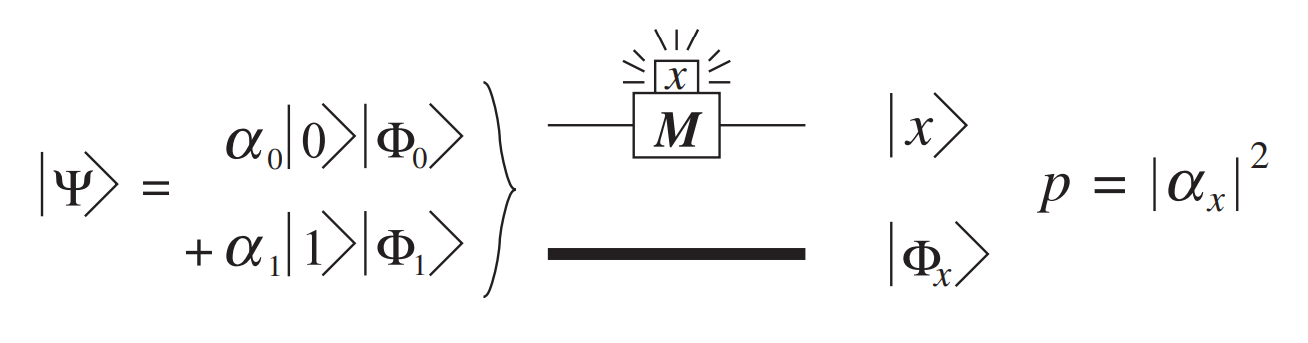
\includegraphics[scale=0.25]{measurement}
\end{figure}

The stronger form of the Born rule applies when one measures only a single one of $n+1$ Qbits by sending it through a standard 1-Qbit measurement gate. The general form of the $(n+1)$ Qbits is given by
\begin{align}
\ket{\Psi}_{n+1} = \sum^{2^{n+1}-1}_{x=0}\gamma(x)\ket{x}_{n+1}, \quad \sum^{2^{n+1}-1}_{x=0}\abs{\gamma(x)}^2 = 1
\end{align}
from which we write explicitly as a combination of the measured Qbit and the other $n$ Qbits:
\begin{align}
\ket{\Psi} = \alpha_0\ket{0}\ket{\Phi_0}_n + \alpha_1 \ket{1}\ket{\Phi_1}_n
\end{align}
where
\begin{align}
\ket{\Phi_0}_n = \f{1}{\alpha_0}\sum^{2^{n}-1}_{x=0}\gamma(x)\ket{x}_n; \quad 
\ket{\Phi_1}_n = \f{1}{\alpha_1}\sum^{2^{n}-1}_{x=0}\gamma(2^n+x)\ket{x}_n
\end{align}
and of course to normalize things
\begin{align}
\alpha^2_0 = \sum^{2^n-1}_{x=0}\abs{\gamma(x)}^2, \quad \alpha^2_1 = \sum^{2^n-1}_{x=0}\abs{\gamma(2^n + x)}^2.
\end{align}
Note that $\ket{\Phi_0}_n$ and $\ket{\Phi_1}_n$ are not necessarily orthogonal.\\

In plain English, the rule asserts that if one measures only the single Qbit whose state symbol is explicitly separated out from the other $n$ Qbits, then the measurement gate will produce $x$ (0 or 1) with probability $\abs{\alpha_x}^2$. The resulting state vector will be the product state $\ket{x}\ket{\Phi_x}_n$. \\

If the Qbit being measured is initially unentangled with the other $n$ Qbits, then the action of the measurement gate on the measured Qbit is just that specified by the Born rule. The unmeasured Qbits are as if they are not there and remain in their original states throughout the process. 

\begin{figure}[!htb]
	\centering
	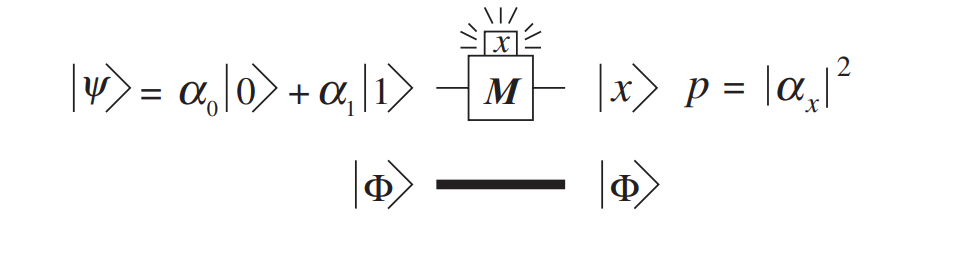
\includegraphics[scale=0.25]{measurement1}
\end{figure}

Applying the generalized Born rule $n$ times to successive 1-Qbit measurements of each of $n$ Qbits initially in $\ket{\psi}_n$, one can show that the final state is $x$ with probability $\abs{\alpha_x}^2$.  Hence, there is only a single primitive piece of measurement hardware: the 1-
Qbit measurement gate. \\

Even more generally, suppose we have the general state of $m+n$ Qbits:
\begin{align}
\ket{\psi}_{m+n} = \sum^{2^m}_{x=0}\alpha_x\ket{x}_m\ket{\Phi_x}_n
\end{align}
where $\sum_x\abs{\alpha_x}^2 = 1$ and the states $\ket{\Phi_x}$ are normalized but not necessarily orthogonal. Applying the Born rule $m$ times to $m$ Qbits we see that if just $m$ Qbits ($\ket{x}_m$) are measured, then with probability $\abs{\alpha_x}^2$ the result will be $x$, and the resulting state vector will be the product state $\ket{x}_m\ket{\Phi_x}_n$.


\subsection{Measurement gates and state preparation}

The measurement gate is useful for producing states with definite states. A measurement that registers $x$ outputs a state in the classical basis $\ket{x}_n$. If we then $\X$ each Qbit that registered a 1 in the measurement and do nothing to the Qbits that registered a 0 then the resulting Qbits will be in the state $\ket{0}_n$. Most quantum-computational algorithms take this state as its input. \\

Measurement gates therefore plays two role: \textit{state preparation} and extracting information from the Qbits. 


\subsection{Constructing arbitrary 1- and 2-Qbit states}

We will first consider the case for a single Qbit. Let $\ket{\psi}$ be any 1-Qbit state, and let $\ket{\phi}$ be an orthogonal state, i.e. $\braket{\psi}{\phi} = 0$. The state $\ket{\phi}$ is unique up to an overall phase. Because $\ket{0}$ and $\ket{1}$ are linearly independent, there is a unique linear transformatin taking them into $\ket{\psi}$ and $\ket{\phi}$. Also, because $\ket{\phi}$ and $\ket{\psi}$ are orthonormal, this linear transformation must be unitary. We will call it $\mathbf{u}$, where
\begin{align}
\ket{\psi} = \mathbf{u}\ket{0}.  
\end{align}
By showing the existence of such a unitary gate $\mathbf{u}$, we're done. \\

Any arbitrary unentangled 2-Qbit state, which is just a fancy way to say it is a tensor product of two 1-Qbit states, can be constructed out of $\ket{00}$ by applying a tensor product of two unitaries to each of the $\ket{0}$ individual states. This follows from the previous argument. To sum this up, we say that an unentangled state requires an unentangled gate to prepare. \\

When the 2-Qbit state is entangled, however, its production requires a 2-Qbit gate that is not a tensor product of two single-Qbit unitaries. The solution, as it turns out, is using a combination of a single cNOT gate and some 1-Qbit unitaries. Consider the general 2-Qbit state:
\begin{align}
\ket{\Psi} = \alpha_{00}\ket{00} + \alpha_{01}\ket{01} + \alpha_{10}\ket{10} + \alpha_{11}\ket{11}.
\end{align}
Observe that this can be re-written in the following way:
\begin{align}
\ket{\Psi} = \ket{0}\otimes \ket{\psi} + \ket{1}\otimes\ket{\phi}
\end{align}
where $\ket{\phi} = \alpha_{00}\ket{0} + \alpha_{01}\ket{1}$ and $\ket{\phi} = \alpha_{10}\ket{0} + \alpha_{11}\ket{1}$.  \\

Next, consider a unitary $\mathbf{u}$ whose action on the computational basis is the following:
\begin{align}
\mathbf{u}\ket{0} = a\ket{0} + b\ket{1}, \quad \mathbf{u}\ket{1} = -b^*\ket{0} + a^*\ket{1}
\end{align}
where $\abs{a}^2 + \abs{b}^2=  1$, as usual. Applying $\mathbf{u}\otimes \Id$ to $\ket{\Psi}$, we get
\begin{align}
\lp\mathbf{u}\otimes \Id\rp \ket{\Psi} &= \lp a\ket{0} + b\ket{1}  \rp\otimes\ket{\psi} +  \lp -b^*\ket{0} + a^*\ket{1}\rp\otimes\ket{\phi}\nn\\
&= \ket{0}\otimes \ket{\psi'} + \ket{1}\otimes \ket{\phi'}
\end{align}
where
\begin{align}
\ket{\psi'}= a\ket{\psi} - b^*\ket{\phi}; \quad \ket{\phi'} = b\ket{\psi} + a^*\ket{\phi}.
\end{align}
Now, if $\ket{\psi'}$ and $\ket{\phi'}$ are orthogonal, then we're done. We wish to choose complex numbers $a,b$ to achieve this. Consider the inner product of $\ket{\psi'}$ and $\ket{\phi'}$:
\begin{align}
\braket{\phi'}{\psi'} = a^2\braket{\phi}{\psi} - b^2\braket{\phi}{\phi} + {ab^*\lp \braket{\psi}{\psi} - \braket{\phi}{\phi} \rp}
\end{align}
If $\braket{\psi}{\phi} \neq 0$ then setting $\braket{\phi'}{\psi'}$ to 0 gives an quadratic equation for the ratio $a/b^*$ = 0, for which there are two complex solutions. Setting $a$ determines a $\mathbf{u}$ for which
\begin{align}
\lp \mathbf{u}\otimes \Id \rp\ket{\Psi} = \ket{0}\otimes\ket{\psi'} + \ket{1}\otimes\ket{\phi'}
\end{align} 
where $\braket{\psi'}{\phi'} = 0$. If $\braket{\phi}{\psi} =0$ then there's nothing else for us to do. $\mathbf{u} \equiv \Id$. \\

Let $\lambda, \mu$ be positive reals such that 
\begin{align}
\ket{\psi''} = \f{\ket{\psi'}}{\lambda}, \quad \ket{\phi''} = \f{\ket{\phi'}}{\mu}
\end{align}
are normalized. This makes $\ket{\psi''}$ and $\ket{\phi''}$ an orthonormal pair. Following an argument earlier, there exists a unitary $\mathbf{v}$ for which 
\begin{align}
\ket{\psi''} = \mathbf{v}\ket{0}, \quad \ket{\phi''} = \mathbf{v}\ket{1}.
\end{align} 
From here, we see that 
\begin{align}
\ket{\Psi} = \lp \mathbf{u}^\dagger \otimes \mathbf{v} \rp\lp \lambda\ket{0}\otimes \ket{0} + \mu\ket{1}\otimes \ket{1} \rp.
\end{align}
Now, note that $\mathbf{C}_{10}\ket{00} \to \ket{00}$ and $\mathbf{C}_{10}\ket{10} \to \ket{11}$. So we can write the equality as follows
\begin{align}
\ket{\Psi} = \lp \mathbf{u}^\dagger \otimes \mathbf{v} \rp \mathbf{C}_{10} \lp \lambda\ket{0} + \mu\ket{1}\rp\otimes \ket{0}.
\end{align}
But we're not finished. Remember that we wish to obtain $\ket{\Psi}$ from $\ket{00} = \ket{0}\otimes \ket{0}$. However, we're very close now, as we only need to obtain $\lambda\ket{0} + \mu\ket{1}$ from $\ket{0}$. Fortunately, we already know how to do this! Consider another unitary $\mathbf{w}$ for which 
\begin{align}
\mathbf{w}\ket{0} = \lambda\ket{0} + \mu\ket{1}
\end{align}
whose existence is guaranteed by our earlier arguments. So, with a single cNOT and three unitaries, we can prepare any entangled 2-Qbit state from $\ket{00}$ via
\begin{align}
\ket{\Psi} = \lp \mathbf{u}^\dagger \otimes \mathbf{v} \rp \mathbf{C}_{10}\lp\mathbf{w}\otimes \Id\rp\ket{00}.
\end{align}












\newpage



\section{Examples}


\subsection{The general computational process}
\subsection{Deutsch's problem}
\subsection{Why additional Qbits needn't mess things up}
\subsection{The Bernstein-Vazirani problem}
\subsection{Simon's problem}
\subsection{Constructing Toffoli gates}


\newpage


\section{Breaking NSA encryption}

\subsection{Preiod finding, factoring, and cryptography}
\subsection{Number-theoretic preliminaries}
\subsection{RSA encryption}
\subsection{Quantum period finding: preliminary remarks}
\subsection{The quantum Fourier transform}
\subsection{Eliminating the 2-Qbit gates}
\subsection{Finding the period}
\subsection{Calculating the periodic function}
\subsection{The unimportance of small phase errors}
\subsection{Period finding and factoring}


\newpage

\section{Searching with a quantum computer}

\subsection{The nature of the search}
\subsection{The Grover iteration}
\subsection{How to construct $\mathbf{W}$}
\subsection{Generalization to several special numbers}
\subsection{Searching for one out of four items}


\newpage

\section{Quantum error correction}

\subsection{The miracle of quantum error correction}
\subsection{A simplified example}
\subsection{The physics of error generation}
\subsection{Diagnosing error syndromes}
\subsection{The 5-Qbit error-correcting code}
\subsection{The 7-Qbit error-correcting code}
\subsection{Operations on 7-Qbit codewords}
\subsection{A 7-Qbit encoding circuit}
\subsection{A 5-Qbit encoding circuit}

\newpage

\section{Protocols that use just a few Qbits}

\subsection{Bell states}
\subsection{Quantum cryptography}
\subsection{Bit commitment}
\subsection{Quantum dense coding}
\subsection{Teleportation}
\subsection{The GHZ puzzle}











\chapter{Quantum Information \& Quantum Computation}
\newpage




\chapter{Problems}

\newpage

\section{Problem Set 1}



\noindent \textbf{1. Computational complexity.}  As mentioned in class, improved algorithms can vastly reduce
the number of required gates (or steps) needed to perform a calculation. In class I used the
example of the bubble sort versus the heap sort and the straightforward discrete Fourier
transform versus the fast Fourier transform. In both of those examples the difference in
complexity of the algorithm was $N^2$ vs. $N \log N$, where for those problems $N$ was the number
of elements that be sorted or the number of points in a time-series. With the algorithmic
change of scaling with $N$ the difference in number of operations becomes huge as $N$ gets
large, but both $N^2$ and $N \log N$ are polynomial in $N$ and the solution is considered \textit{efficiently
computable} with either algorithm.
\\

To think more about what is meant by not being efficiently computable, you will now consider
the goal of finding prime factors of a (large) composite number. The basic idea of finding
prime factors is that given an integer $n$-bit integer $N$ find a factorization
\begin{align}
N = pq
\end{align}
where at least one of the integers $p$ and $q$ are prime.
\begin{enumerate}[(a)]
	\item The most straightforward algorithm for finding prime factors is called ``trial division'' or
	``direct-search factorization'' and it is just what it sounds like. Start testing all integers
	up to $p = \sqrt{N}$ as possible factors. A number $N$ is represented by a binary number
	with $n = \lg(N)$ bits. Show that this leads to an exponential scaling in the number of
	bits $\mathcal{O}(2^{n/2})$, which is exponential in the number of bits. This is still the most efficient algorithm for relatively small numbers.
	\item  As mentioned in class the most efficiently known classical factoring algorithm for large
	numbers is the ``number field sieve'' and its complexity is $\mathcal{O}\lp e^{cn^{1/3}(\ln n )^{2/3}}  \rp$, where $c =
	(64/9)^{1/3}$, which is also exponential in the number of bits. Shor’s quantum algorithm is $\mathcal{O}(n^3)$ which is polynomial in $n$, and thus is efficient. Create a table showing the
	difference in the number of steps (time) needed to factor an n-bit number using these
	four methods for $n =$ 4, 16, 32, 64, 128, 256, 512, and 1024. The RSA challenge for RSA-768 a 768 bit (232 decimal digit) number was factored in
	2009 using the number field sieve after several years using ``many hundreds of machines.''
	A similar effort factored RSA-240 (795 bits) in 2019
\end{enumerate}


\noindent \textit{Solution:} 
\begin{enumerate}[(a)]
	\item Let a number $N$ be given. $N$ is represented by a binary number with $n = \lg(N)$ bits. The trial division algorithm tests integers up to $p = \sqrt{N}$, which can be represented by a binary number with $\tilde{n} = \lg(\sqrt{N}) = n/2$. It follows that the number of test integers (from 1 to $p$) is on the order of $2^{n/2}$. This means there is an exponential scaling in the number of bits $\mathcal{O}\lp 2^{n/2} \rp$. 
	\item 
	$\,$\\
	\begin{tabular}{|c|c|c|}
		\hline
		n & $\exp\lc \sqrt[3]{64/19}\sqrt[3]{n}(\ln n)^{2/3}  \rc$ & $n^3$\\
		\hline
		4&$19.3$&$64$\\
		16&$1730$&$4096$\\
		32&$5.41\times 10^4$&$3.28 \times 10^4$\\
		64&$5.43\times 10^6$&$2.62 \times 10^5$\\
		128&$2.53\times 10^9$&$2.10 \times 10^6$\\
		256&$8.92\times 10^{12}$&$1.68 \times 10^7$\\
		512&$4.46\times 10^{17}$&$1.34 \times 10^8$\\
		1024&$7.16\times 10^{23}$&$1.07\times 10^9$\\
		\hline
	\end{tabular}
\end{enumerate}
\qed




\newpage





\noindent \textbf{2. Reversible Computation.} Quantum computation is reversible. That is, no matter how
sophisticated the computation is, you can always run the program in reverse and figure out
what was input to start the computation. In 1973 Charles Bennett (IBM) showed that you
could perform any classical computation using reversible gates, and reversible computation
has been a part of theoretical computer-science since then. The NOT gate is reversible, but
the standard two-CBit gates, AND, OR, and XOR, are clearly not reversible because they
have two inputs and only one output so you can’t recreate their inputs knowing their outputs.








\begin{enumerate}
	\item \textit{Controlled-not (CNOT)}. While the standard exclusive-or (XOR, $\oplus$) gate of Boolean logic
	is not reversible, there is a reversible equivalent to the XOR gate called the controlled-not (CNOT) gate. As shown below in both the circuit diagram and the truth table it
	has two inputs and two outputs.
	\begin{figure}[!htb]
		\centering
		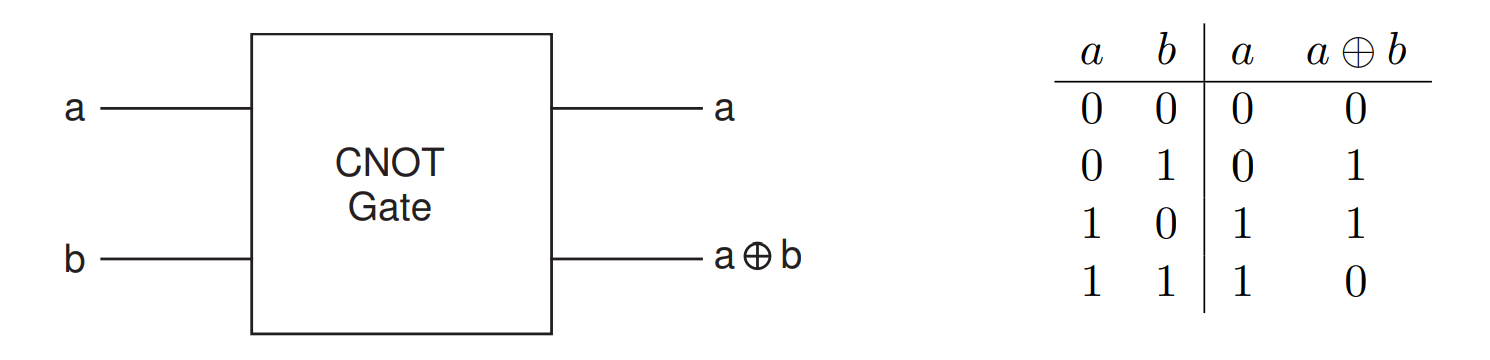
\includegraphics[scale=0.25]{cnot}
	\end{figure}
	Show by creating the truth table that the CNOT gate is reversible - that you can find
	the inputs if you know the outputs. In fact, you can show that CNOT is its own inverse.
	To do this you will ``prove'' the identity $a \oplus (a \oplus b) = b$.

	
	\item \textit{Toffoli Gate}. While the CNOT gate is reversible, it is not universal. That is, you cannot
	implement every possible logic operation with the CNOT. The NAND gate is actually
	\textit{universal}: you can create any logical operation using just NAND gates (but of course
	it isn’t reversible). In 1980 Tommaso Toffoli (MIT) described a universal reversible
	gate – now called the Toffoli gate or sometimes the ``controlled-controlled-not.'' [There’s
	another universal reversible gate called the Fredkin gate (or ``controlled-swap'') named
	after its inventor Edward Fredkin.] The Toffoli gate has three inputs and three outputs
	and its behavior is shown in the circuit diagram shown below. The outputs are a copy
	of both inputs and the logical expression $c \oplus (a \land b)$.
	\begin{figure}[!htb]
		\centering
		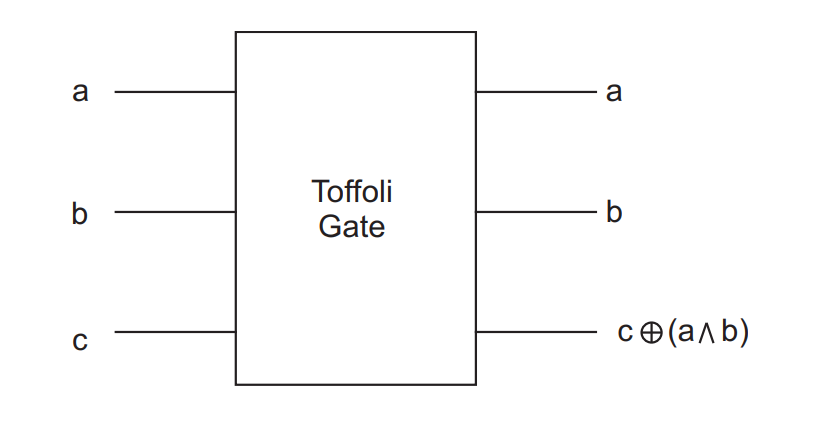
\includegraphics[scale=0.25]{toffoli}
	\end{figure}
	There are 8 possible input combinations to the Toffoli gate. Create a truth table for the
	Toffoli gate and show that for $c = 0$ that the output is $a \land b$ and for $c = 1$ that the output
	is $a \land b$ where $\land$ is the symbol for AND. That is, show the Toffoli gate can generate the
	same logical output as the AND or NAND gates.
	Show that the Toffoli gate is its own inverse by creating the truth table using the three
	outputs you calculated as inputs to a Toffoli gate.
	Why would the Toffoli gate be called the controlled-controlled-not (CCNOT)?
\end{enumerate}


\noindent \textit{Solution:} 
\begin{enumerate}[(a)]
	\item 
	$\,$CNOT:\\
	\begin{tabular}{| c  c |  c c| c| }
		\hline
		$a$ & $b$ & $a$ & $a\oplus b$  & $a\oplus(a\oplus b)$ \\
		\hline
		0&0&0&0&0\\
		0&1&0&1&1\\
		1&0&1&1&0\\
		1&1&1&0&1\\
		\hline
	\end{tabular}

	We have just shown (by exhaustion) that $a\oplus(a\oplus b) = b$, which means we can invert the CNOT gate to obtain its input $(a,b)$ for any given output $(a,a\oplus b)$. 
	
	\item 
	$\,$Toffoli:\\
	\begin{tabular}{| c  c  c  c| c c c| }
		\hline
		$a$ & $b$ & $c$ & $(a\land b)$ & $a$ & $b$&  $c\oplus (a\land b)$ \\
		\hline
		0&0&0&0&0&0&0\\
		0&0&1&0&0&0&1\\
		0&1&0&0&0&1&0\\
		0&1&1&0&0&1&1\\
		1&0&0&0&1&0&0\\
		1&0&1&0&1&0&1\\
		1&1&0&1&1&1&1\\
		1&1&1&1&1&1&0\\
		\hline
	\end{tabular}

	We see that $\text{Toff}[a,b,0]=a\land b$, and $\text{Toff}[a,b,1] = \overline{a\land b}$. So, by setting $c$ to be $0$ or $1$, we can make the Toffoli gate an AND or a NAND gate. \\
	
	To show that the Toffoli gate is its own inverse, we show $c = (a\land b) \oplus c\oplus (a\land b)$, once again by exhaustion:\\
	
	\begin{tabular}{| c  c  c  c| c c c| c |}
		\hline
		$a$ & $b$ & $c$ & $(a\land b)$ & $a$ & $b$&  $c\oplus (a\land b)$ & $(a\land b) \oplus c\oplus (a\land b)$  \\
		\hline
		0&0&0&0&0&0&0&0\\
		0&0&1&0&0&0&1&1\\
		0&1&0&0&0&1&0&0\\
		0&1&1&0&0&1&1&1\\
		1&0&0&0&1&0&0&0\\
		1&0&1&0&1&0&1&1\\
		1&1&0&1&1&1&1&0\\
		1&1&1&1&1&1&0&1\\
		\hline
	\end{tabular}

	The Toffoli gate would be called the controlled-controlled-not because unlike the CNOT where there is one control bit and one target bit, the Toffoli gate has \textbf{two} control bits, namely $a$ and $b$, and one target bit, namely $c$. The Toffoli gate flips $c$ if and only if $a = b = 1$. 
	
\end{enumerate}


\qed


\newpage
\noindent \textbf{3.} In Section 1.4, Mermin defines several 1-Cbit operations that do not correspond to any physical operation but which can be useful in deriving relationships between operations that do
have a physical meaning. The first two of these operators are the ``projection operators.'' 

\begin{figure}[!htb]
	\centering
	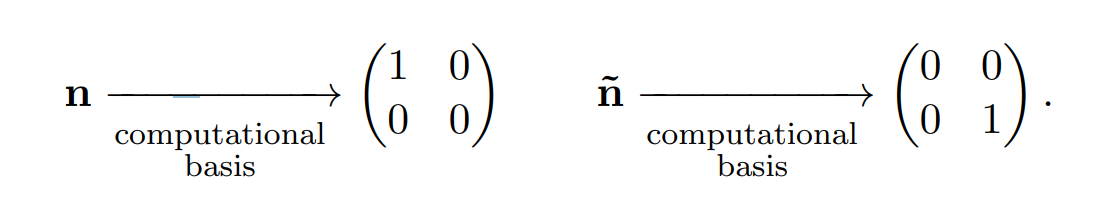
\includegraphics[scale=0.3]{proj}
\end{figure}
\begin{enumerate}[(a)]
	\item Show, using their matrix form, that as Mermin states on the top of page 12, the two
	matrices have eigenvalues of 0 and +1. Determine eigenvectors of each matrix assuming
	that they are in the form of probabilistic CBits
	\begin{align*}
	\ket{a} = \begin{pmatrix}
	a_0 \\ a_1
	\end{pmatrix}
	\end{align*}
	where the convention of probability requires $a_0 + a_1 = 1$. 
	
	\item Show, using the definitions, that the properties of Eq. 1.33 and 1.34 are correct.
	
\end{enumerate}


\noindent \textit{Solution:} 
\begin{enumerate}[(a)]
	\item Because $\mathbf{n}$ and $\tilde{\mathbf{n}}$ are diagonal matrices with only entries $0$ and $1$ along the diagonals, their eigenvalues are 0 and 1. \\
	
	The (stochastic) 1-eigenvector of $\mathbf{n}$, say $\ket{a}_1= (a_0\,\,a_1)^\top$ where $a_0 + a_1 = 1$, must be ${\ket{a}_1 = (1\,\,0)^\top}$ because $\mathbf{n}(a_0\,\,a_1)^\top = (a_0\,\,0)^\top$. By a similar argument, the (stochastic) 0-eigenvector of $\mathbf{n}$ must be ${\ket{a}_0 = (0\,\,1)^\top}$. By symmetry, the 1-eigenvector of $\tilde{\mathbf{n}}$ is ${\ket{\tilde{a}}_{{1}} = (0\,\,1)^\top}$, and the 0-eigenvector of $\tilde{\mathbf{n}}$ is ${\ket{\tilde{a}}_{{0}} = (1\,\,0)^\top}$.
	
	\item We note that projections are \textit{idempotents}, so $\mathbf{n}^2 = \mathbf{n}$ and $\tilde{\mathbf{n}}^2 = \tilde{\mathbf{n}}$ automatically. Next, because the images of $\mathbf{n}$ and $\tilde{\mathbf{n}}$ are orthogonal spaces (spanned by $(1\,\,0)^\top$ and $(0\,\,1)^\top$, respectively), $\mathbf{n}\tilde{\mathbf{n}} = \tilde{\mathbf{n}}\mathbf{n} = \mathbf{0}_{2\times 2}$. Finally, $\mathbf{n} + \tilde{\mathbf{n}} = \Id$ because the idempotents $\mathbf{n}$ and $\tilde{\mathbf{n}}$ \textit{resolve identity} $\Id$. \\
	
	We can also verify these properties algebraically:
	\begin{align}
	&\mathbf{n}^2 = \begin{pmatrix}
	1&0\\0&0
	\end{pmatrix}\begin{pmatrix}
	1&0\\0&0
	\end{pmatrix} = \begin{pmatrix}
	1&0\\0&0
	\end{pmatrix}\\
	&\tilde{\mathbf{n}}^2 = \begin{pmatrix}
	0&0\\0&1
	\end{pmatrix}\begin{pmatrix}
	0&0\\0&1
	\end{pmatrix}=\begin{pmatrix}
	0&0\\0&1
	\end{pmatrix}\\
	&\mathbf{n}\tilde{\mathbf{n}}= \begin{pmatrix}
	1&0\\0&0
	\end{pmatrix}
	\begin{pmatrix}
	0&0\\0&1
	\end{pmatrix} = \begin{pmatrix}
	0&0\\0&0
	\end{pmatrix} = \begin{pmatrix}
	0&0\\0&1
	\end{pmatrix}\begin{pmatrix}
	1&0\\0&0
	\end{pmatrix} = \tilde{\mathbf{n}}\mathbf{n}\\
	&\mathbf{n} +  \tilde{\mathbf{n}}  = \begin{pmatrix}
	1&0\\0&0
	\end{pmatrix} + \begin{pmatrix}
	0&0\\0&1
	\end{pmatrix} = \begin{pmatrix}
	1&0\\0&1
	\end{pmatrix} = \Id
	\end{align} 
	
	Next we consider the $\X = \begin{pmatrix}
	0&1\\1&0
	\end{pmatrix}$, the bit-flip:
	\begin{align}
	&\mathbf{n}\X = \begin{pmatrix}
	1&0\\0&0
	\end{pmatrix}\begin{pmatrix}
	0&1\\1&0
	\end{pmatrix}= \begin{pmatrix}
	0&1\\0&0
	\end{pmatrix}=\begin{pmatrix}
	0&1\\1&0
	\end{pmatrix}\begin{pmatrix}
	0&0\\0&1
	\end{pmatrix} = \mathbf{X}\tilde{\mathbf{n}}\\
	&\tilde{\mathbf{n}}\X = \begin{pmatrix}
	0&0\\0&1
	\end{pmatrix}\begin{pmatrix}
	0&1\\1&0
	\end{pmatrix}= \begin{pmatrix}
	0&0\\1&0
	\end{pmatrix}=\begin{pmatrix}
	0&1\\1&0
	\end{pmatrix}\begin{pmatrix}
	1&0\\0&0
	\end{pmatrix} = \mathbf{X}{\mathbf{n}}.
	\end{align}
	Mermin explained why this makes sense, so I won't repeat that.
	
	
\end{enumerate}

\qed













\newpage
\noindent \textbf{4.} Another pair of operators which do not have physical meaning when acting on CBits are the
``phase-flip operator'' $\mathbf{Z}$ and Hadamard operator $\had$. 
\begin{figure}[!htb]
	\centering
	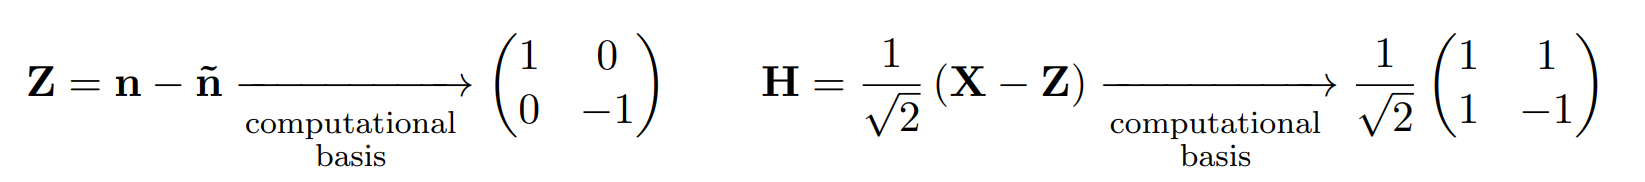
\includegraphics[scale=0.26]{ZH}
\end{figure}
where $\X$ is the ``bit-flip'' (NOT) operator. Both $\mathbf{Z}$ and $\had$ will be used and do have meaning when applied to QBits.

\begin{enumerate}[(a)]
	\item Show, using their matrix forms, that the three single-bit gates $\X$, $\mathbf{Z}$, and $\had$ are their
	own inverse. That is, show that $\X^2 = \Id$, $\mathbf{Z}^2 = \Id$, and $\had^2 = \Id$.
	\item Show, using their matrix forms, that the identities of Eq. 1.43 are correct. That is, show
	that using a Hadamard gate to perform a ``similarity transformation'' you can convert a bit-flip to a phase-flip and vice-versa.
\end{enumerate}

\noindent \textit{Solution:} 

\begin{enumerate}[(a)]
	\item 
	\begin{align}
	\mathbf{Z}^2 &= \begin{pmatrix}
	1&0\\0&-1
	\end{pmatrix}\begin{pmatrix}
	1&0\\0&-1
	\end{pmatrix} = \begin{pmatrix}
	1&0\\0&1
	\end{pmatrix}\\
	\X^2 &= \begin{pmatrix}
	0&1\\1&0
	\end{pmatrix}\begin{pmatrix}
	0&1\\1&0
	\end{pmatrix} = \begin{pmatrix}
	1&0\\0&1
	\end{pmatrix}\\
	\had^2 &= \f{1}{2}\begin{pmatrix}
	1&1\\1&-1
	\end{pmatrix}\begin{pmatrix}
	1&1\\1&-1
	\end{pmatrix} = \begin{pmatrix}
	1&0\\0&1
	\end{pmatrix}.
	\end{align}
	
	\item 
	\begin{align}
	\had \X \had &= \f{1}{2}\begin{pmatrix}
	1&1\\1&-1
	\end{pmatrix}\begin{pmatrix}
	0&1\\1&0
	\end{pmatrix}\begin{pmatrix}
	1&1\\1&-1
	\end{pmatrix} = \begin{pmatrix}
	1&0\\0&-1
	\end{pmatrix} = \mathbf{Z}\\
	\had \X\had &= \mathbf{Z} \implies \X = \had^{-1}\mathbf{Z}\had^{-1}  \implies \X = \had \mathbf{Z} \had \quad (\had^{-1} = \had) 
	\end{align}
\end{enumerate}
\qed
















\end{document}